% main.tex -- top-level document. Compile this.
%
%   pdflatex main && pdflatex main      (twice, for \ref resolution)
%
% Each section lives in its own file and is \input below. Sections contain no
% preamble and no \documentclass; everything shared lives here.
%
% FIGURES. Every figure is currently a \figspec placeholder: a framed box
% carrying its own plot specification, so this document compiles with an empty
% figures/ directory. To land a real plot, replace
%     \figspec{4.2cm}{...spec text...}
% with
%     \includegraphics[width=\columnwidth]{figures/NAME}
% and leave the \caption and \label alone. Delete the \figspec macro once no
% call sites remain.
%
% NOT COMPILED -- no LaTeX toolchain was available where this was assembled.
% Checked statically for brace/environment balance, escaping, dangling
% references and table column counts. Treat the first build as proofreading.

\documentclass[10pt,twocolumn]{article}

\usepackage[margin=0.75in]{geometry}
\usepackage[T1]{fontenc}
\usepackage[utf8]{inputenc}
\usepackage{booktabs}
\usepackage{amsmath}
\usepackage{amssymb}
\usepackage{xspace}
\usepackage{graphicx}
\usepackage{algorithm}
\usepackage{algpseudocode}
\usepackage[hidelinks]{hyperref}

\graphicspath{{figures/}}

% ---------------------------------------------------------------- macros ---
\newcommand{\sysname}{Tandem\xspace}   % system name; change here only

% Placeholder standing in for an unrendered plot. #1 optional width,
% #2 box height, #3 the plot specification.
\newcommand{\figspec}[3][0.95\columnwidth]{%
  \fbox{\parbox[c][#2][c]{#1}{\centering\footnotesize\itshape #3}}}

\title{\sysname: Arbitrating Model and Data Residency\\
       for Agentic HPC Workflows}
\author{}
\date{}

\begin{document}
\maketitle

\input{01_intro}
\section{Background and Related Work}

\subsection{Traditional vs.\ Agentic Scientific Workflows}

High Performance Computing workflows consist of multi-stage applications that
produce and manipulate data in multiple discrete phases to produce an end
result or insight. A phase typically corresponds to a computational task
(e.g., a simulation, analysis, or visualization step) that consumes data
produced by previous phases and generates data for subsequent ones. For
instance, a workflow meant to discover new alloys could involve preparing
alloy structures in one phase, running Density Functional Theory calculations
on each, and then aggregating and visualizing the data. Sometimes these phases
may be cyclical, with phases repeating in a set order, where the outputs of
one series of phases become the inputs to the next. Common high-impact HPC
workflows include protein and alloy discovery, astronomical simulation, and
fluid dynamics workflows. The use of these workflows to simulate, analyze, and
derive insights from data has led to significant advances in multiple
scientific fields, including the discovery of new proteins for medical
applications, analysis and identification of cosmological phenomena such as
supernovae in massive telescope data streams, and rapid speed-ups of
prototyping for fluid-dependent systems in fields such as aerospace
engineering.

\subsection{Prior Solutions for Memory Bottlenecks}

Despite their advantages for scientific progress, HPC workflows face a key
challenge: their operations on massive datasets lead to an imbalance between
the efficiency of compute hardware and memory bandwidth. Workflows often
involve multi-GB datasets that can balloon quickly as simulation steps produce
more data from their initial inputs (e.g., 100,000 atoms having their energy
interactions for every 1~ns step simulated by a protein folding program). This
data can easily make an HPC workflow's data ``out-of-core'' for part or all of
a workflow, meaning the data is too large to fit in RAM all at once. This
results in data movement costs, and the infamous ``memory wall'': hardware
FLOPs have scaled $60000\times$ in the past 20 years, while DRAM bandwidth has
only scaled $100\times$ and interconnect bandwidth $20\times$ in the same
timespan. While some HPC sites have addressed this by scaling their DRAM, the
financial and energy cost of this scaling makes it unsustainable.

In recent work, the solution to this issue has come in the form of software
distributed shared memory (DSM) systems that present tiered memory and storage
resources as an ``infinite memory pool'', often referred to as a Deep Memory
and Storage Hierarchy (DMSH). This system relies on the predictable
phase-based nature of HPC workflows in order to handle both the organization
of data across the memory and storage hierarchy and ensure coherency without
infeasible overhead. Information about phase intent and accesses allows data to
be staged proactively, placed across the hierarchy intelligently, and
prefetched while other computation is running to ensure no idle computational
resources. For example, if a simulation phase is known to consume a particular
trajectory, a DMSH data staging system can begin loading that data from
storage while the preceding analysis phase is still executing, hiding most of
the I/O latency behind computation. Intent and expected accesses are
transmitted to the system via API.

\subsection{Workload Description}

\paragraph{AtomAgents.}
AtomAgents is a multi-agent materials discovery framework built on AutoGen
that combines LLM reasoning with physics-based simulation tools such as
LAMMPS. Specialized agents collaborate to plan, execute, and refine scientific
workflows by invoking simulation tools through function-calling interfaces.
Each tool invocation represents a workflow phase whose required simulation
inputs, intermediate datasets, and even successor phases are determined only
after the agents complete their reasoning.

% NOTE: five sentences in this section arrived truncated from the source
% document (mid-word cuts at "an oracle-informed retention policy because...",
% "Adding accelerator capacity th models...", "roughly 86% of the total problem
% disappears...", "A sta construction cost as fits...", and "The two mechanisms
% are thus that vary in practice..."). They are restored below and marked with
% % RESTORED so they can be checked against intent.

\section{Gaps, Insights and Opportunities}

\subsection{Agents Break Existing HPC DMSH Solutions}

\paragraph{Agents Create Workflow Nondeterminism.}
Although their impact on scientific goals is significant, AI-steered HPC
workflows break a fundamental assumption made by memory-storage software DSM
systems about scientific HPC workflows: that of predictable phases and data
accesses. AI steering agents make independent choices about which data will be
used for computation in an upcoming phase (and in some cases even about which
phases will be triggered). As a result, prior systems that treat storage as an
extension of memory are unable to prefetch the correct data for each step in
agentic HPC workflows because they rely on the definition of deterministic
phases in an HPC workflow program. This leads to stalls while the required
data is fetched from storage into memory. Figure~\ref{fig:predictability}
demonstrates the proportion of runs of the same workflow that deviate from the
most common action taken at a given step index. With only 30--60\% agreement
at any given step, it exemplifies that even given the exact same task to
investigate, agentic frameworks will produce significantly different behavior.
Functionally, agentic workflows are not deterministic.

\begin{figure}[t]
\centering
% PLOT SPEC (kept for provenance; rendered by
% scripts/figures/make_figures.py -> figure_drafts/fig-predictability.pdf)
%   $x$ = step index, $y$ = share of runs taking the modal action at that 
%   step, over repeated executions of an identical task. Band the 30--60\% 
%   region. Optionally overlay a second series for a second workflow to show 
%   the pattern is not workload-specific.
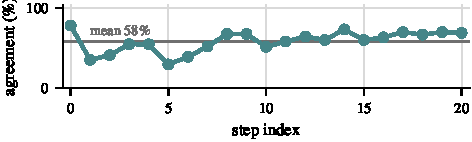
\includegraphics[width=\columnwidth]{figures/fig-predictability}
\caption{Agreement with the modal action at each step index across repeated
executions of an identical task. Agreement never exceeds 60\%, so the same
request produces materially different executions.}
\label{fig:predictability}
\end{figure}

\paragraph{Agents Add Memory Pressure.}
To make matters worse, the core problem these solutions address is compounded
in AI-steered workflows because AI agents comprise multi-billion-parameter
models requiring anything from 2--200~GB of space (for most common models).
The loading of model weights from disk all the way to GPU VRAM is some of the
most expensive loading work in a workflow, and as such agentic workflows
typically offload models that may be reused later onto CPU RAM. However, this
means models are now in competition with the scientific data they work with
for the RAM resources available, exacerbating the memory pressure HPC
workflows experience. Figure~\ref{fig:replacement-loss} shows a visual
workflow timeline against the page cache hits of a workflow over time, showing
how typical ``weight-parking'' behavior can cycle useful data out of RAM.

\begin{figure}[t]
\centering
% PLOT SPEC (kept for provenance; rendered by
% scripts/figures/make_figures.py -> figure_drafts/fig-replacement-loss.pdf)
%   two aligned panels sharing an $x$ axis of wall time. Top: workflow 
%   timeline with model-load, model-park and tool-invocation spans. Bottom: 
%   page-cache hit rate (or resident bytes) for the scientific artifact. 
%   Annotate the points where a park event is followed by a collapse in the 
%   artifact's residency and a subsequent re-read.
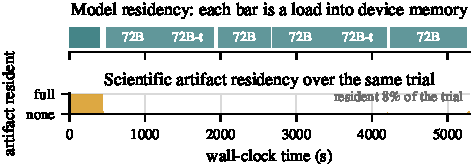
\includegraphics[width=\columnwidth]{figures/fig-replacement-loss}
\caption{Model parking evicts scientific data. Each parking event coincides
with a loss of the artifact's residency, which the next tool invocation must
pay to rebuild.}
\label{fig:replacement-loss}
\end{figure}

\paragraph{Agents Rely Heavily On Data Transformations.}
Data used by agentic tools must undergo a representation change. A
representation change is work that produces a structure the consumer could not
have obtained by placing bytes. In other words, if the in-memory structure the
consumer requires is byte-identical to some contiguous range of the
file---modulo a header---then making it usable is placement. Otherwise the
structure is a computed function of the file, and producing it is a
representation change. These representation changes are responsible for 93\%
on average of the stalls caused by waiting for data staging. Because the
product of a representation change is a computed structure rather than a range
of a file, it cannot be named, staged, or evicted by a byte-oriented tier at
all: it exists only as anonymous memory inside a live consumer process. Parked
model weights have the same property, for the same reason. The ceiling on a
placement-oriented system is therefore set by which rungs of the cost chain
its interface can reach, not by how accurately it predicts---no improvement in
prediction moves a cost the interface cannot express. And because the retained
structure and the parked model both occupy anonymous memory drawn from a
single allocation, the question these workflows pose is not which bytes to
fetch but which structures to keep, and---when they cannot all be kept---which
of them a gigabyte of memory is better spent on.

\subsection{Value-Ranking Opportunities}

\paragraph{Not Every GB Retained Is Equally Valuable.}
If retention is the action, a scheduler needs a price: how many seconds of
future stall a gigabyte of held memory buys. That price is not uniform, and it
is non-uniform in a way that rules out any fixed policy. Holding logical
content fixed---the same array, bit for bit, in six serialisations---the
seconds saved per gigabyte retained span $65\times$, from 22.0 for ASCII
numeric text to 0.34 for a memory-mappable binary layout
(Figure~\ref{fig:sgb-spread}). Model weights occupy a far narrower band of
2.78--3.81, and for a structural reason: a model's cost is dominated by moving
bytes at roughly fixed bandwidth, so it is near-linear in size and its price
per gigabyte is nearly constant. Data has no such anchor, because the cost of
a representation change is set by the decoder rather than by the byte count.

The consequence is that models land in the middle of the data range rather
than above or below it. Some artifacts are worth an order of magnitude more
per gigabyte than any model; others are worth almost nothing. A fixed class
priority---models first, or data first---is therefore wrong at one end of the
range or the other, and the correct ordering is recoverable only by pricing
each resource individually.

Two properties make that pricing practical. First, the price is a property of
the representation rather than of the instance: across a $4\times$ size range
it is flat to within 1.00--1.16$\times$, so it can be measured once per format
and reused without profiling. Second, there is a floor. Materialising any
structure into a process address space costs roughly 0.32~s/GB regardless of
format, so a resource whose price approaches that floor performs no
transformation at all, and retaining it buys nothing that placement would not.

\begin{figure}[t]
\centering
% PLOT SPEC (kept for provenance; rendered by
% scripts/figures/make_figures.py -> figure_drafts/fig-sgb-spread.pdf)
%   seconds saved per GB retained, log $y$, one point per resource. Shade 
%   the narrow model band (2.78--3.81) as a horizontal strip; scatter the 
%   data artifacts across it, from ASCII at 22.0 to memory-mappable binary 
%   at 0.34. Draw a horizontal rule at the 0.32~s/GB materialisation floor. 
%   The models-in-the-middle geometry is the reading.
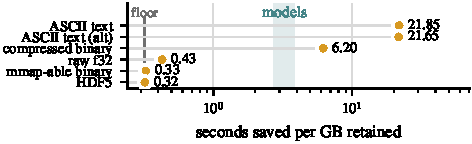
\includegraphics[width=\columnwidth]{figures/fig-sgb-spread}
\caption{Retention value per gigabyte across resources. Models occupy a narrow
band set by transfer bandwidth; data artifacts span $65\times$ and bracket
that band on both sides, so no fixed class priority is correct.}
\label{fig:sgb-spread}
\end{figure}

\paragraph{Value-Aware Retention vs.\ Prefetching Depend on Hardware Topology
and the Inter-need Gap.}
Retention and speculative staging are not two implementations of one idea;
they serve disjoint populations of stalls. Retention can only help a resource
used more than once---a first use has nothing to retain---while staging is the
only mechanism that can help a first use at all. Which dominates is therefore
set by reuse density: resource needs per distinct resource.

That quantity moves with scale. Holding schedule length fixed and growing the
resource population from 5 to 28, the share of needs that are first uses rises
from 10.4\% to 32.3\%, and the advantage shifts correspondingly from retention
toward staging (Figure~\ref{fig:scale-sweep}). The shift is structural rather
than a matter of prediction quality: an oracle-informed retention policy fades
over the same range, because the misses it could convert are progressively not
there to convert.  % RESTORED

Hardware topology moves the balance a second way, and in both directions.
Accelerator capacity and host memory are separate budgets, and a model
actively resident on an accelerator charges neither. Adding accelerator
capacity therefore removes precisely the models most worth retaining, leaving
a less-used remainder to compete for host memory and shrinking what
value-aware arbitration can recover.  % RESTORED
Host memory behaves symmetrically: once the budget is large enough that
nothing is ever evicted---in our configuration at roughly 86\% of the total
footprint---the arbitration problem disappears and retaining everything is
correct.  % RESTORED
Budget also buys value in steps rather than smoothly, since additional memory
pays only when it crosses a threshold admitting one more resource
(Figure~\ref{fig:topology-budget}).

Finally, the inter-need gap bounds what staging can achieve. A stage recovers
only as much of a construction cost as fits into the window before the need
arrives, so the same mechanism captures more as computation between tool calls
grows.  % RESTORED
Retention has no such dependence---its saving is the full construction cost
whenever the resource is next used. The two mechanisms are thus complementary
along both axes that vary in practice, which is the case for arbitrating them
jointly rather than choosing one.  % RESTORED

\begin{figure}[t]
\centering
% PLOT SPEC (kept for provenance; rendered by
% scripts/figures/make_figures.py -> figure_drafts/fig-scale-sweep.pdf)
%   $x$ = number of distinct resources (5, 10, 18, 28). Left axis: advantage 
%   over the recency-ranked baseline for retention and for staging, as two 
%   lines that cross. Right axis: first-use share, rising 10.4\% 
%   $\rightarrow$ 32.3\%. The crossing is the reading.
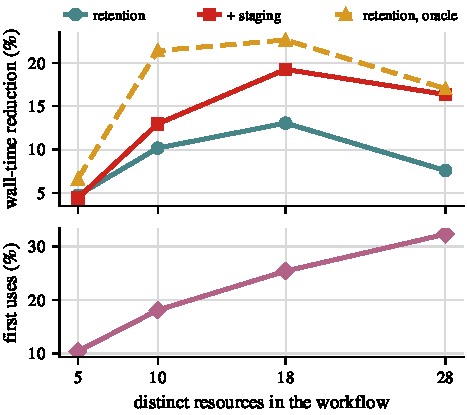
\includegraphics[width=\columnwidth]{figures/fig-scale-sweep}
\caption{As the resource population grows at fixed schedule length, first uses
become a larger share of all needs and the advantage moves from retention to
staging.}
\label{fig:scale-sweep}
\end{figure}

\begin{figure}[t]
\centering
% PLOT SPEC (kept for provenance; rendered by
% scripts/figures/make_figures.py -> figure_drafts/fig-topology-budget.pdf)
%   $x$ = budget as \% of total footprint. $y$ = share of decisions in which 
%   memory pressure forced an eviction, one line per accelerator-slot count, 
%   falling to zero. Mark the packing thresholds with vertical rules so the 
%   step structure is visible. This is the motivating view; 
%   Figure~\ref{fig:budget-sweep} shows the same axis with performance 
%   rather than pressure.
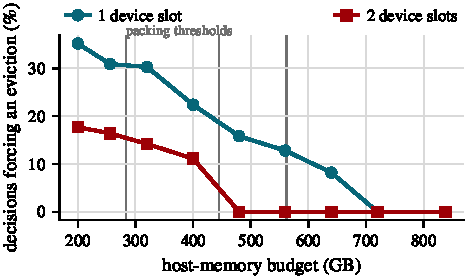
\includegraphics[width=\columnwidth]{figures/fig-topology-budget}
\caption{Contention as a function of budget and accelerator capacity. Above
roughly 86\% of the total footprint nothing is ever evicted and the
arbitration problem disappears; below it, budget admits resources in steps
rather than smoothly.}
\label{fig:topology-budget}
\end{figure}

\subsection{Speculative Value-Ranking Opportunities}

\paragraph{Local transition structure survives workflow-level nondeterminism.}
Agentic workflows are dynamic in the large but structured in the small: tools
exhibit high-confidence $k$-offset successor relationships, in which one tool
consistently follows another a fixed number of invocations later. Not every
tool has such a successor at every offset, but nearly every tool has one at
some offset. Figure~\ref{fig:tool-relationships} shows this for AtomAgents at
both framework and workflow level---restricting to $k \in [0,5]$, both
workflows contain numerous relationships with empirical confidence between 0.9
and 1.0. Critically, these relationships persist across substantially
different prompts and objectives within a framework, so traces from prior,
unrelated executions supply useful priors on the first run of a workflow never
seen before.

\paragraph{Plans predict order, not distance.}
Frameworks organised by a planner agent expose a second, longer-range signal:
a natural-language plan naming the tools to be invoked and their intended
order. In AtomAgents these plans predict 95\% of tool orderings correctly
(Figure~\ref{fig:plan-accuracy}), far enough ahead to begin staging resources
whose construction would otherwise be exposed. What they do not supply is
distance: agents insert additional calls to recover from syntax errors and
retry failures, so the observed trace diverges from the planned offsets even
when the order is right. Plans therefore reach far but locate poorly, while
local transitions locate well but do not reach---which is why the two are used
together.

\begin{figure}[t]
\centering
% PLOT SPEC (kept for provenance; rendered by
% scripts/figures/make_figures.py -> figure_drafts/fig-tool-relationships.pdf)
%   heatmap or matrix, source tool $\times$ offset $k \in [0,5]$, cell 
%   shaded by the confidence of the highest-confidence successor at that 
%   offset. Two panels: framework level and workflow level. Highlight cells 
%   in the 0.9--1.0 band. The reading is that nearly every row has at least 
%   one dark cell.
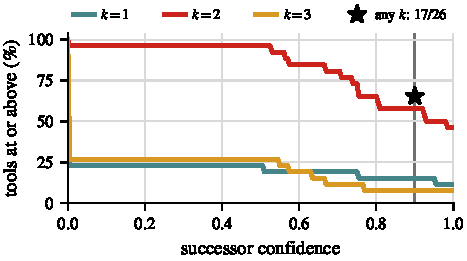
\includegraphics[width=\columnwidth]{figures/fig-tool-relationships}
\caption{High-confidence $k$-offset successor relationships in AtomAgents.
Nearly every tool has at least one successor at some offset with confidence
above 0.9, despite workflow-level nondeterminism.}
\label{fig:tool-relationships}
\end{figure}

\begin{figure}[t]
\centering
% PLOT SPEC (kept for provenance; rendered by
% scripts/figures/make_figures.py -> figure_drafts/fig-plan-accuracy.pdf)
%   planned tool order versus realized tool order. Either (a) a 
%   confusion-style plot of planned rank versus realized rank, or (b) paired 
%   bars for ordering accuracy (95\%) against offset-distance accuracy (much 
%   lower). Option (b) makes the order-vs-distance contrast, which is the 
%   point of the paragraph.
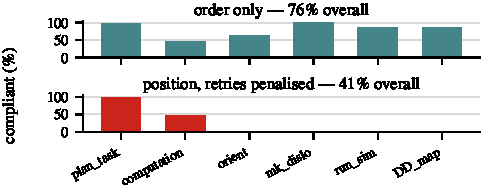
\includegraphics[width=\columnwidth]{figures/fig-plan-accuracy}
\caption{Planner-declared orderings are accurate; planner-implied distances
are not. Agents insert recovery and retry calls, so realized offsets diverge
from planned ones even when the order is correct.}
\label{fig:plan-accuracy}
\end{figure}

\input{04_system}
% NUMBERS. Simulation results come from sc-workshop-paper/results_tables/*.md,
% regenerated by scripts/make_results_tables.py; the prose cites cells, not
% hand-copied constants, so swapping simulation for measurement means re-running
% that script and re-reading the same cells:
%
%   Stall Reduction     -> 02_budget_sweep.md
%   End-to-End Runtime  -> 02_budget_sweep.md, 03_compute_sweep.md
%   DMSH comparison     -> results/eval_q1_q4/eval_q1_summary.csv (MEASURED),
%                          faceted to gpu_name == "NVIDIA L40S"; stall classes
%                          from eval_stall_taxonomy.csv. The ONLY measured
%                          end-to-end subsection. Do not let it be pooled
%                          across accelerator generations.
%   Ablations           -> 01_attribution_ladder.md, 06_prefetch_variants.md
%   CPU interference    -> results/bench_preactivation_interference.json and
%                          results/bench_potential_activation_rusage_*.json
%                          (both MEASURED)
%   Sensitivity         -> 07_objective_check.md, 02_budget_sweep.md,
%                          04_accuracy_sweep.md
%
% OPEN ITEM: the exact-selection column of 04_accuracy_sweep.md runs deeply
% negative at 560 GB / 2 slots. The system specifies a predictor reporting "not
% within H" rather than "never"; those cells appear to have been generated
% WITHOUT that bounded-lookahead reporting, so they may measure an arm the
% design does not describe. The exact arm is omitted from the prose below until
% that is resolved.

\section{Evaluation}

\subsection{Setup}

Results are trace-driven simulation over measured resource constants. Park
footprints, cold-boot and wake costs, activated sizes and per-format
construction rates are measured on hardware; schedules and the clock are
synthetic. Each reported value averages 3 popularity orderings $\times$ 2
schedule populations $\times$ 10 schedules of 48 resource needs. The
comparison against a byte-oriented tiering system
(Section~\ref{sec:dmsh}) is measured end-to-end and is marked as such.

We report against two baselines. \textsc{Never} retains nothing: a displaced
model is terminated and a data artifact is reconstructed on every use. It is
the honest denominator for the mechanism. \textsc{Lru} retains both classes
but ranks by recency alone; it is already a system, so it is the line any
policy claim must clear. Reporting only against \textsc{Never} would credit
arbitration for benefits that plain retention already delivers.

\subsection{Stall Reduction}

At the production 256~GB allocation with a single device slot, \textsc{Lru}
removes 26.97\% of the \textsc{Never} baseline's wall time and \sysname
removes 34.49\%, eliminating a further 11.55\% of the stall \textsc{Lru}
leaves behind (Figure~\ref{fig:stall-ladder}). The margin widens as the budget
admits more of the working set: at 560~GB with two slots \sysname removes
50.69\% of \textsc{Lru}'s residual stall.
Figure~\ref{fig:budget-sweep} shows the effect across the full budget range,
together with the fraction of decisions in which memory pressure actually
forced an eviction. That fraction is the more informative axis: it falls from
35.2\% at 200~GB to 0.0\% by 720~GB, and where it reaches zero the correct
policy is to retain everything and no arbitration is required. Budget also
buys performance in steps rather than smoothly, since additional memory is
only useful when it crosses a threshold admitting one more resource---which is
why 320~GB and 400~GB perform almost identically.

\begin{figure}[t]
\centering
\figspec{4.2cm}{\textbf{fig:stall-ladder} --- grouped bars, stall seconds per
arm (\textsc{Never}, \textsc{Lru}, \sysname) at 256~GB/1 slot and
560~GB/2 slots. Annotate each \sysname bar with its reduction over
\textsc{Lru}.}
\caption{Stall attributable to resource residency, by policy and
configuration. \sysname removes 11.55\% of the stall \textsc{Lru} leaves at
the production allocation and 50.69\% at a larger budget.}
\label{fig:stall-ladder}
\end{figure}

\subsection{End-to-End Runtime}

\sysname reduces end-to-end wall time by 34.49\% against \textsc{Never} and
10.30\% against \textsc{Lru} at 256~GB with one device slot, rising to 50.81\%
and 17.09\% respectively with two (Figure~\ref{fig:budget-sweep}).

These wall-clock figures are a function of how much real computation the
workload performs between tool invocations, and we report that dependence
rather than a single number (Figure~\ref{fig:compute-sweep}). Holding the
mechanism fixed and varying only the inter-need gap, the wall-clock reduction
over \textsc{Lru} falls from 10.56\% at 5.7\% compute to 6.99\% at 54.9\% and
0.89\% at 95.1\%, purely because the denominator grows. The stall reduction
moves the opposite way over the same sweep---11.21\%, 15.49\%,
18.24\%---because a larger compute window hides more of each staging
operation. Our measured workload sits near the low-compute end, spending
280.3~s of a 5288.5~s trial on agent work, so we attach the compute share to
every wall-clock claim.

\begin{figure*}[t]
\centering
\figspec[0.95\textwidth]{5.0cm}{\textbf{fig:budget-sweep} --- two panels, one
per device-slot count. $x$ = budget (200--838~GB). Lines: \textsc{Lru} and
\sysname, both as \% reduction vs \textsc{Never}. Twin right-hand axis:
binding \% (share of decisions that forced an eviction), shaded. Mark the
packing thresholds at 283, 445, 562 and 838~GB with vertical rules --- the
step structure is the point.}
\caption{Wall-time reduction versus budget and device capacity. The shaded
series is the fraction of decisions in which memory pressure forced an
eviction; where it reaches zero the arbitration problem has disappeared and
retaining everything is correct.}
\label{fig:budget-sweep}
\end{figure*}

\begin{figure}[t]
\centering
\figspec{4.2cm}{\textbf{fig:compute-sweep} --- $x$ = compute share of wall
(5.7\%--95.1\%, log). Two lines vs \textsc{Lru}: wall-clock reduction
(falling) and stall reduction (rising). Mark the measured workload's operating
point near 5\%. The crossing behaviour is the reading.}
\caption{The same mechanism reported two ways. Wall-clock reduction is diluted
by compute; stall reduction improves with it, because a longer window hides
more of a staging operation.}
\label{fig:compute-sweep}
\end{figure}

\subsection{Comparison with Byte-Oriented Tiering}
\label{sec:dmsh}

Unlike the rest of this section, the results here are measured end-to-end on
hardware rather than simulated.

We compare against a state-of-the-art DMSH system on a workflow selected for
contrast: its inter-step gaps are short, so there is structurally very little
opportunity to overlap staging with computation. The DMSH arms ran only on
L40S nodes, so every row of Table~\ref{tab:dmsh} is restricted to that
partition. Pooling accelerator generations is not admissible here---identical
work has been measured to differ by up to $2.3\times$ across node types---and
the pooled figure would overstate the contrast.

\begin{table}[t]
\centering\small
\begin{tabular}{@{}lrrrl@{}}
\toprule
Configuration & $n$ & Wall (s) & $\times$base & Dominant stall class \\
\midrule
Baseline            & 9 & $270.8 \pm 52.3$  & 1.00 & no prefetch \\
\sysname            & 9 & $300.4 \pm 61.8$  & 1.11 & \texttt{no\_window} \\
DMSH, informed      & 7 & $862.2 \pm 230.9$ & 3.18 & \texttt{window\_too\_small} \\
DMSH, random        & 7 & $796.4 \pm 90.0$  & 2.94 & \texttt{window\_too\_small} \\
\bottomrule
\end{tabular}
\caption{Measured end-to-end wall time on L40S nodes for the short-window
workload. The DMSH system's informed and random staging variants are
statistically indistinguishable from one another.}
\label{tab:dmsh}
\end{table}

The DMSH system increases end-to-end wall time by $3.18\times$, and the
increase is unambiguous ($t = +6.65$). More informative than the magnitude is
the reason. Every stall it incurs classifies as \texttt{window\_too\_small}:
the system identified data to stage and began staging it, but the interval
before the need was too short to complete the transfer. Consistent with that
diagnosis, replacing its staging decisions with random ones does not make it
worse---the two variants are statistically indistinguishable ($t = +0.70$).
The failure is therefore not mis-prediction, which better prediction would
address, but the absence of a window, which it would not.

The same workload bounds what any staging-based approach can achieve on it:
an oracle arm with perfect hindsight still classifies 100\% of its stalls as
\texttt{no\_window}. \sysname is not statistically separable from the
unmodified baseline here ($t = +1.10$, on a point estimate 11\% higher), which
is the intended behaviour---where there is no window to exploit and little
reuse to retain, the system should cost approximately nothing rather than pay
for speculation that cannot repay it. We report this workload precisely
because it is the adverse case for our own mechanism as well as for the
baseline we compare against.

\subsection{Ablations}

We decompose the result by adding one mechanism at a time
(Figure~\ref{fig:ablation}). At 256~GB with one device slot, parking models
alone accounts for 5.64\%; adding retention of activated data reaches 26.97\%;
cost-aware arbitration adds 5.90 points to 32.87\%; and slack staging adds a
further 1.62 to 34.49\%. Because marginal credit depends on the order in which
mechanisms are added, we also report an order-independent Shapley
decomposition of the retention total: at this budget model parking accounts
for 2\% and data retention for 98\%, since neither of the two largest models
fits the budget at all. At 560~GB the same decomposition gives 61\% and 39\%,
so the split is a property of the allocation rather than of the system, and we
report it with the budget attached.

A second ablation varies what a wrong staging decision is permitted to destroy
(Figure~\ref{fig:prefetch-variants}). At measured predictor accuracy,
restricting staging to slack yields $+10.30$\% over \textsc{Lru} while
permitting displacement yields $+5.91$\%; restricting scope to data artifacts
yields $+13.10$\%. The safety rule matters more than the scope restriction,
and neither is a better predictor---both simply bound the cost of being wrong.

\begin{figure}[t]
\centering
\figspec{4.6cm}{\textbf{fig:ablation} --- horizontal cumulative bar,
\textsc{Never} $\rightarrow$ +model parking $\rightarrow$ +data retention
$\rightarrow$ +cost-aware arbitration $\rightarrow$ +slack staging, annotated
with each marginal contribution. Inset or second panel: Shapley split of the
retention total at 256~GB and 560~GB, showing the reversal.}
\caption{Contribution of each mechanism at 256~GB with one device slot, and
the order-independent split of the retention total at two budgets.}
\label{fig:ablation}
\end{figure}

\begin{figure}[t]
\centering
\figspec{4.2cm}{\textbf{fig:prefetch-variants} --- grouped bars at measured
accuracy: retain-only, data+slack, data+outbid, all+slack, all+outbid, as \%
vs \textsc{Lru}. Optionally repeat at two accuracies to show the safety rule's
stability.}
\caption{Two independent restrictions on speculative staging: which classes it
may stage, and whether it may displace a retained resource.}
\label{fig:prefetch-variants}
\end{figure}

\subsection{Performance Penalties of Processes on CPU for Foreground Work}

Retention and staging both consume CPU in resident worker processes, so we
measured whether that work degrades the foreground agent
(Figure~\ref{fig:cpu-interference}). With 0, 1, 2, 4 and 8 concurrent
background construction processes, foreground median latency was 0.618, 0.618,
0.617, 0.618 and 0.618~s---slowdowns of 1.000, 0.999, 0.997, 1.000 and 1.000.

A perfectly flat curve is also the signature of a probe that silently did
nothing, so we instrumented the run rather than accepting it: eight workers
were alive, load average reached 7.25, and the workers consumed 46.41
CPU-seconds in 6~s of wall time. They genuinely ran.

The result follows from construction being single-threaded, which we confirm
directly---a full artifact construction consumes 0.9885 CPU-seconds per second
of wall time. Each staging task is therefore exactly one core, and staging
tasks do not contend with one another. The practical consequence is that the
arbitrator budgets memory only, which is what makes value per gigabyte a
complete decision variable rather than one term of a two-resource trade-off.

This holds where tested, and we state the boundary. Every level measured was
under-subscribed---at most nine active processes on twelve cores---with
working sets of roughly 78~MB. Memory-bandwidth contention at the scale of a
fully activated artifact, three orders of magnitude larger, is not exercised
by this experiment.

\begin{figure}[t]
\centering
\figspec{4.2cm}{\textbf{fig:cpu-interference} --- $x$ = concurrent background
construction processes (0,1,2,4,8). Left axis: foreground median latency,
flat. Right axis: CPU-seconds consumed by the workers, rising. Plot both ---
the flatness is only credible next to evidence the workers ran.}
\caption{Foreground latency under concurrent background construction. The
rising CPU-seconds series is reported alongside the flat latency series
because a null result and a broken probe are otherwise indistinguishable.}
\label{fig:cpu-interference}
\end{figure}

\subsection{Sensitivity Sweeps}

\paragraph{Horizon.}
Retention is insensitive to $H$ across a wide range, varying by 0.14 points
between $H=60$~s and $H=600$~s, while staging degrades steadily once $H$
exceeds the workload's typical inter-need gap: 67.75\% at $H=60$, 62.19\% at
$H=600$, and 55.07\% at $H=3000$ (Figure~\ref{fig:h-sweep}). The asymmetry is
expected---$H$ exists to keep near-term candidates comparable on absolute
savings, and enlarging it past the window in which a staging operation can
complete admits candidates that cannot pay off. Setting $H$ near the observed
inter-step gap is sufficient; no tuning beyond that order of magnitude was
required.

\paragraph{Hardware topology.}
We sweep device slots against budget (Figure~\ref{fig:budget-sweep}). A second
device slot substantially raises absolute performance but reduces the value of
host-memory arbitration, because the models worth retaining are already
resident on the device and what competes for host memory is the less-used
remainder. Arbitration therefore matters most where device capacity is scarce
relative to the number of distinct models in the workflow.

\paragraph{Predictor accuracy.}
Figure~\ref{fig:accuracy-sweep} sweeps horizon accuracy from 0.15 to 1.00.
Retention is essentially flat, moving from $+7.50$\% to $+7.99$\% over
\textsc{Lru}, since horizon error perturbs a ranking rather than forcing a
selection. Slack staging degrades gracefully, from $+5.65$\% to $+18.72$\%,
and remains positive throughout: an operation that consumes only unclaimed
memory cannot destroy a retention worth more, so its downside is bounded by
wasted bandwidth. Permitting displacement removes that bound, and the same
sweep runs from $-6.22$\% at 0.15 accuracy to $+19.67$\% at 1.00, which is the
quantitative basis for the conjunctive conditions the outbid path carries in
Section~\ref{sec:prefetch}.

\begin{figure}[t]
\centering
\figspec{4.2cm}{\textbf{fig:h-sweep} --- $x = H$ (60--3000~s, log). Two
lines: retention (flat) and retention+staging (declining). Shade the region
around the workload's median inter-need gap.}
\caption{Sensitivity to the planning horizon $H$. Retention is insensitive;
staging degrades once $H$ exceeds the window in which a stage can complete.}
\label{fig:h-sweep}
\end{figure}

\begin{figure}[t]
\centering
\figspec{4.2cm}{\textbf{fig:accuracy-sweep} --- $x$ = horizon accuracy
(0.15--1.00). Three lines vs \textsc{Lru}: retention (flat), slack staging
(rising, always $>0$), outbid staging (crossing zero near 0.35). Mark the
measured accuracy band. The zero crossing is the reading.}
\caption{Sensitivity to horizon accuracy. Retention and slack staging remain
beneficial across the range; only displacement-permitting staging is
accuracy-critical.}
\label{fig:accuracy-sweep}
\end{figure}


\end{document}
